\documentclass{../../slides-style}

\slidetitle{Введение в Linux}{01.03.2024}

\begin{document}
    
    \begin{frame}[plain]
        \titlepage
    \end{frame}

    \section{Что такое Linux и зачем он нам}

    \begin{frame}{Linux --- что это и зачем?}
        \begin{itemize}
            \item Linux --- семейство Unix-подобных операционных систем
            \begin{itemize}
                \item Есть сотни дистрибутивов (из которых десяток только широкоизвестных), на базе более-менее общего ядра
                \item \url{https://github.com/torvalds/linux}
            \end{itemize}
            \item С открытым исходным кодом, широкое сообщество разработчиков
            \item В основном для серверов, встроенных устройств и всякого странного оборудования
            \begin{itemize}
                \item На волне импортозамещения популяризуется и для конечных пользователей
            \end{itemize}
            \item Удобнее для программирования
            \item Хуже для игр, хуже с поддержкой железа
        \end{itemize}
    \end{frame}

    \begin{frame}{Linux для программистов}
        \begin{itemize}
            \item Бесплатна
            \begin{itemize}
                \item Поэтому можно ставить на виртуальные машины/контейнеры в любом количестве
                \item В типичном серверном окружении \emph{каждый} процесс работает в своём контейнере, так что лицензии на другие ОС легко разорят кого угодно
                \item Есть нюанс --- целый рынок небесплатных дистрибутивов. Свобода ПО не значит, что на нём нельзя зарабатывать.
            \end{itemize}
            \item Очень конфигурируема --- от полноценных десктопных дистрибутивов до миниатюрных систем в десятки мегабайт
            \item Удобная командная строка
            \item Пакетный менеджер
            \item Некоторые инструменты есть только для Linux
            \begin{itemize}
                \item Valgrind, QEMU, Gem5, ...
                \item Кое-что можно запустить и на Windows, но это нетривиально
            \end{itemize}
        \end{itemize}
    \end{frame}

    \begin{frame}
        \begin{center}
            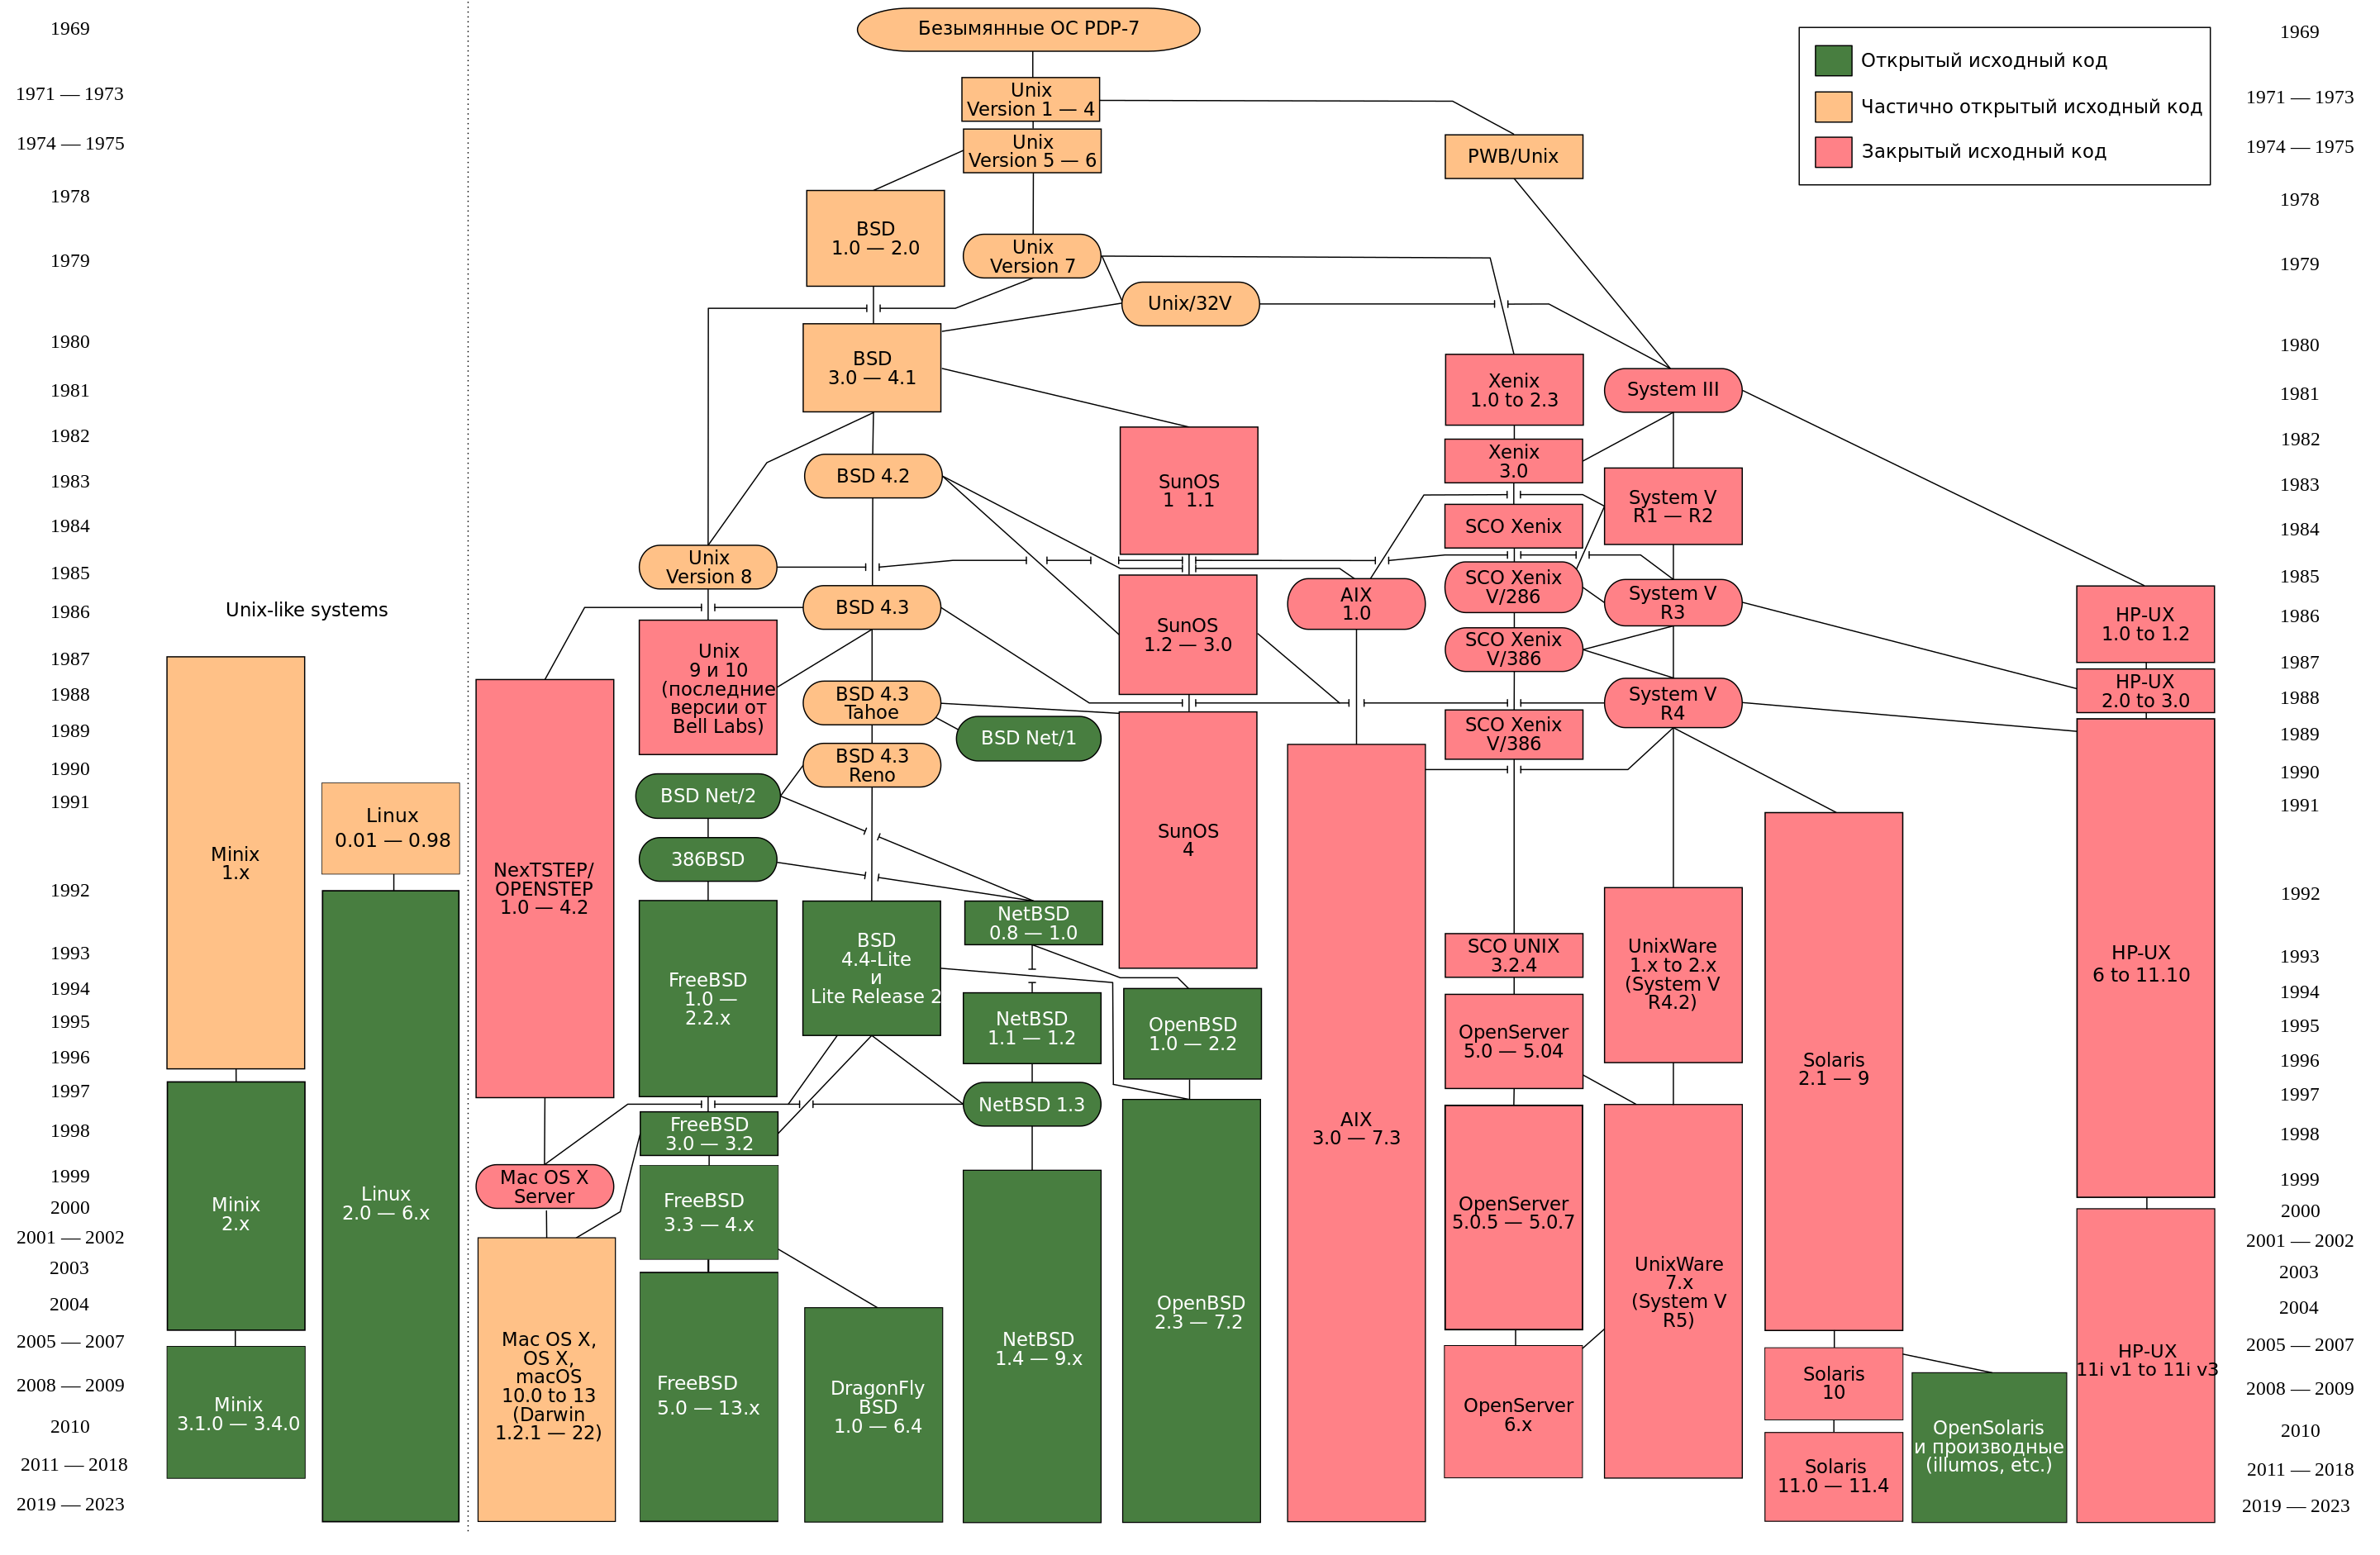
\includegraphics[width=0.95\textwidth]{unixHistory.png}
        \end{center}
    \end{frame}

    \begin{frame}{Отличия от Windows}
        \framesubtitle{С точки зрения пользователя}
        \begin{itemize}
            \item Пакетный менеджер
            \begin{itemize}
                \item Как NuGet, только в масштабах всей системы
                \item Часто старые версии
                \item Специфичен для дистрибутива
                \item Может быть несколько репозиториев пакетов
            \end{itemize}
            \item Регистрозависимая файловая система
            \item Одно дерево файлов, начинающееся в \enquote{/}, монтирование
            \item Много мелких консольных команд, из которых можно собирать сложные штуки
            \item Оконный менеджер --- обычное внешнее приложение
            \item Запускаемое приложение по умолчанию не ищется в текущей папке
            \item Человекочитаемые файлы конфигурации
        \end{itemize}
    \end{frame}

    \section{Что бывает}

    \begin{frame}{Дистрибутивы}
        \begin{itemize}
            \item Дистрибутив --- это готовое к установке ядро, набор программ и пакетная экосистема
            \item Популярные дистрибутивы:
            \begin{itemize}
                \item Ubuntu
                \item Mint
                \item Fedora
                \item Debian
                \item Arch
                \item Gentoo
                \item Альт, РОСА, Астра
            \end{itemize}
            \item Откуда пошли разные дистрибутивы: \url{https://upload.wikimedia.org/wikipedia/commons/1/1b/Linux_Distribution_Timeline.svg}
        \end{itemize}
    \end{frame}

    \begin{frame}{Пакеты}
        \begin{itemize}
            \item Пакет --- способ распространения приложений и библиотек. 
            \item Состоит из метаинформации, бинарников, конфигов, доков, иногда исходников
            \item Дерево зависимостей
            \item Популярные форматы пакетов: deb, rpm
            \item Базовые утилиты: rpm, dpkg
            \item Популярные пакетные менеджеры: 
            \begin{itemize}
                \item apt (Advanced Packaging Tool) --- Debian, Ubuntu, Mint, Альт
                \item yum (Yellowdog Updater, Modified) --- старая Fedora и дистрибутивы на её основе
                \item dnf (Dandified YUM) --- Fedora, РОСА
            \end{itemize}
            \item Формат имени пакета: \mintinline{text}{<название>-<версия>-<выпуск>.<архитектура>}
            \item Альтернативный подход: ставить приложение со всеми зависимостями целиком
            \begin{itemize}
                \item Flatpak, Snappy, AppImage
            \end{itemize}
        \end{itemize}
    \end{frame}

    \begin{frame}{Среды рабочего стола}
        \begin{itemize}
            \item Оконные системы: X Window System, Wayland
            \item Среды рабочего стола
            \begin{itemize}
                \item GNOME (на GTK+) и его производные (MATE, Cinnamon)
                \item KDE (Plasma) (на Qt)
                \item XFCE (на GTK+)
            \end{itemize}
            \item Более-менее исключают друг друга
            \begin{itemize}
                \item Приложение для одной среды запустится в другой, но потащит за собой огромную кучу зависимостей и будет выглядеть \emph{необычно}
            \end{itemize}
            \item Дистрибутивы иногда имеют варианты (Ubuntu --- GNOME, KUbuntu --- KDE)
        \end{itemize}
    \end{frame}

    \section{Работа с консолью --- 1}

    \begin{frame}{Основные консольные команды (1)}
        \begin{itemize}
            \item cd --- переход в директорию
            \begin{itemize}
                \item Абсолютные пути с /
                \item Относительные пути, специальные директории . и ..
            \end{itemize}
            \item pwd --- вывести текущую директорию (обычно в приглашении)
            \item ls --- показать содержимое директории
            \begin{itemize}
                \item Ключи -a, -l
            \end{itemize}
            \item mkdir --- создать директорию
            \begin{itemize}
                \item Ключ -p
            \end{itemize}
            \item touch --- обновить время последнего обращения к файлу или создать пустой файл
            \item echo --- распечатать что-то в консоль
        \end{itemize}
    \end{frame}

    \begin{frame}{Основные консольные команды (2)}
        \begin{itemize}
            \item cat --- вывести содержимое файла на консоль
            \item cp --- скопировать файл/директорию
            \item mv --- переместить файл/директорию
            \item rm --- удалить файл/директорию
            \begin{itemize}
                \item Ключ -rf
            \end{itemize}
            \item ln --- создать ссылку
            \begin{itemize}
                \item Жёсткие и символьные ссылки (ln -s)
            \end{itemize}
            \item sudo --- запустить от имени суперпользователя
        \end{itemize}
    \end{frame}

    \section{Файловая система}

    \begin{frame}{Отвлечение про файловую систему}
        \begin{itemize}
            \item Файловая система суть набор inode (индексный дескриптор)
            \item Посмотреть можно ls -i
            \item Режим доступа: Read, Write, Execute, для владельца, группы, всех
            \begin{itemize}
                \item chmod
            \end{itemize}
            \item Имена файлов живут отдельно от inode-ов
            \item Что-то вроде сборки мусора --- если ни одно имя не указывает на inode, его удаляют
            \item Символьная ссылка --- это путь к файлу, а не inode
            \item Файлы вовсе не обязательно лежат на диске
            \begin{itemize}
                \item Всё, что поддерживает потоковый ввод-вывод --- файл!
                \item /dev/null, /dev/random, /proc/...
            \end{itemize}
        \end{itemize}
    \end{frame}

    \begin{frame}{Filesystem Hierarchy Standard}
        \begin{itemize}
            \item Бывают изменяемые и статичные файлы, и разделяемые и неразделяемые
            \begin{itemize}
                \item Разные условия доступа по сети и бэкапов
                \item Следовательно, должны лежать в разных директориях
            \end{itemize}
            \item Корневая файловая система --- только самое необходимое для загрузки и восстановления системы, к ней подмонтируются другие директории
            \begin{itemize}
                \item Никто не мешает им быть на одном разделе с корневой
                \item Могут быть на других дисках или вообще в сети
            \end{itemize}
            \item Всё не критичное для системы барахло --- в /usr
            \item Запрещено создавать файлы и директории в корне
        \end{itemize}
    \end{frame}

    \begin{frame}{Стандартные директории}
        \begin{itemize}
            \item /bin --- нужные программы (в т.ч. для пользователя)
            \item /boot --- файлы загрузчика
            \item /dev --- файлы устройств (они не лежат на диске, если что)
            \item /etc --- конфиги (не разделяемые)
            \item /lib --- библиотеки и модули ядра
            \item /media --- сюда монтируются внешние носители типа флешек
            \item /mnt --- директория для временного монтирования
            \item /opt --- директория для дополнительных пакетов (обычно проприетарных)
            \item /sbin --- нужные программы (для администратора)
            \item /tmp --- временные файлы
            \item /usr --- вторичная иерархия (примерно та же иерархия, но из некритичных файлов)
            \begin{itemize}
                \item Сейчас популярен \enquote{joined root}, когда bin -> /usr/bin, а /sbin -> /usr/sbin
            \end{itemize}
            \item /var --- изменяемые данные
            \item \dots
        \end{itemize}
    \end{frame}

    \section{Работа с консолью --- 2}

    \begin{frame}{Немного более продвинутая работа с консолью}
        \begin{itemize}
            \item wildcards (globs) --- \mintinline{text}{file[1-8]}, \mintinline{text}{file*}, есть ещё \mintinline{text}{?}, \mintinline{text}{[!]}
            \begin{itemize}
                \item Это те самые глобы из .gitignore
                \item Они раскрываются \emph{до} вызова команды
            \end{itemize}
            \item Сильное и слабое квотирование
            \item Переменные окружения: \mintinline{text}{$PATH}, export
            \item which --- найти программу в путях, whereis --- найти все её файлы
            \item find: \mintinline{text}{find /usr/share/doc -name README}
            \item locate --- ищет и пути
        \end{itemize}
    \end{frame}

    \begin{frame}{Управление процессами}
        \begin{itemize}
            \item Убить процесс --- Ctrl-C
            \item Остановить --- Ctrl-Z (как бы ставит на паузу)
            \item fg и bg, оператор \mintinline{text}{&}
            \item kill, killall --- послать сигнал процессу
            \begin{itemize}
                \item SIGINT, SIGTERM, SIGKILL
            \end{itemize}
            \item ps, top
            \item Перенаправление: \mintinline{text}{>}, \mintinline{text}{>>}, \mintinline{text}{|}
            \begin{itemize}
                \item \mintinline{text}{echo lol > file.txt}
                \item \mintinline{text}{echo lol | wc}
                \item \mintinline{text}{cat file.txt | sort | uniq | wc -l}
            \end{itemize}
        \end{itemize}
    \end{frame}

    \begin{frame}{Работа с текстом}
        \begin{itemize}
            \item sort, uniq, wc
            \item head, tail
            \item more, less
            \item sed, awk
            \item vim
        \end{itemize}
    \end{frame}

    \begin{frame}{Полезные штуки}
        \begin{itemize}
            \item Табуляция
            \item .bashrc, .bash\_profile, alias
            \item Midnight Commander
            \item reverse-i-search (Ctrl-R, Ctrl-S)
            \item Ctrl-W, Ctrl-U
            \item Выделение мышью, вставка средней кнопкой
            \item Клавиша Compose
            \item Ctrl-Alt-F1, Ctrl-Alt-F2 и т.д., Ctrl-Alt-Backspace
            \item Всегда имеет смысл ставить проприетарные драйвера для видеокарты, и они почти никогда не ставятся по умолчанию
        \end{itemize}
    \end{frame}

    \section{Справка}

    \begin{frame}{Документация}
        \begin{itemize}
            \item Стандартизована, в целом лучше поддерживается, чем для типичных Windows-программ
            \item man
            \begin{itemize}
                \item RTFM!
                \item Секции man, 9 разделов, 1 --- пользовательские программы, 2 --- системные вызовы и т.д.
            \end{itemize}
            \item whatis
            \item apropos
            \item info --- более продвинутый формат документации, с гиперссылками
            \item Документация дистрибутива
        \end{itemize}
    \end{frame}

\end{document}